\chapter{Introduction}

\section{Science of Science}
The underlying driving force of science has always been to start from empirical evidence in order to gain information
about the structure of the phenomena taking place around us. With such a pursuit in mind it was just a matter of time until science
would start investigating \textit{itself}. The moment came in the 60s, when the first bibliographic efforts required to improve the searchability of
scientific material took place in the form of a 
search for proper indexing \cite{bibliography_literature,Garfield108}
and therefore allowing, for the first time, to analyze the published material as its own data set. 
With only few previous works being carried out \cite{half_life}, the historical breakthrough in the field of science of science came with De Solla Price's work
\textit{Networks of Scientific Papers} \cite{deSollaPrice510}. De Solla's publication not only was one of the first 
to directly tackle the pattern of bibliographical references, but it also introduced key concepts for the development of the field,
starting from the need to analyze it in its topological structure as a network. Figs.\ref{fig:desolla_network} and \ref{fig:desolla_matrix}
show the earliest attempts of representing citation data as a network, even though the theory behind network science was still in its 
earliest stages. 



\begin{figure}[h!]
\centering
        \setbox0\hbox{%
                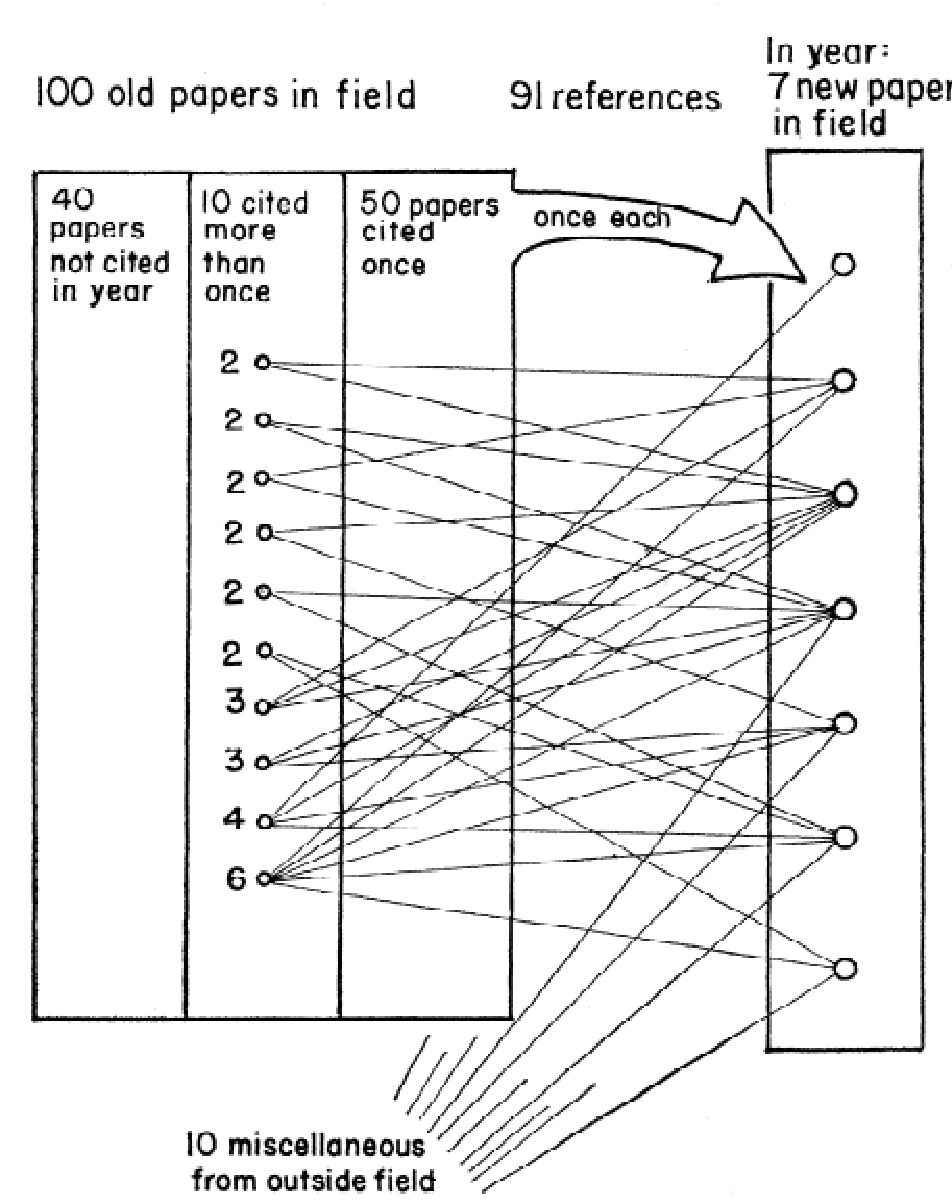
\includegraphics[width=.55\textwidth]{desolla.pdf}%
        }%
        \setbox2\hbox{%
                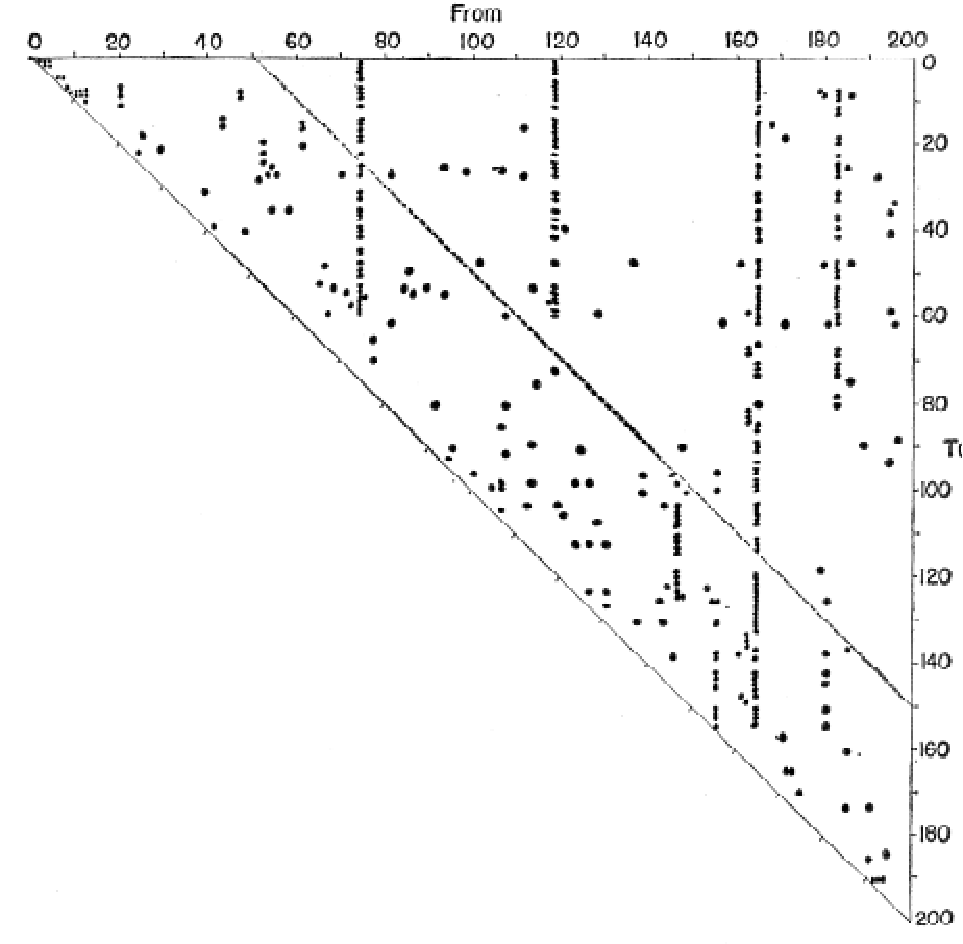
\includegraphics[width=.55\textwidth]{desollaadjacency.pdf}%
        }%
        \ifdim\ht0>\ht2
                \setbox0\hbox{%
                        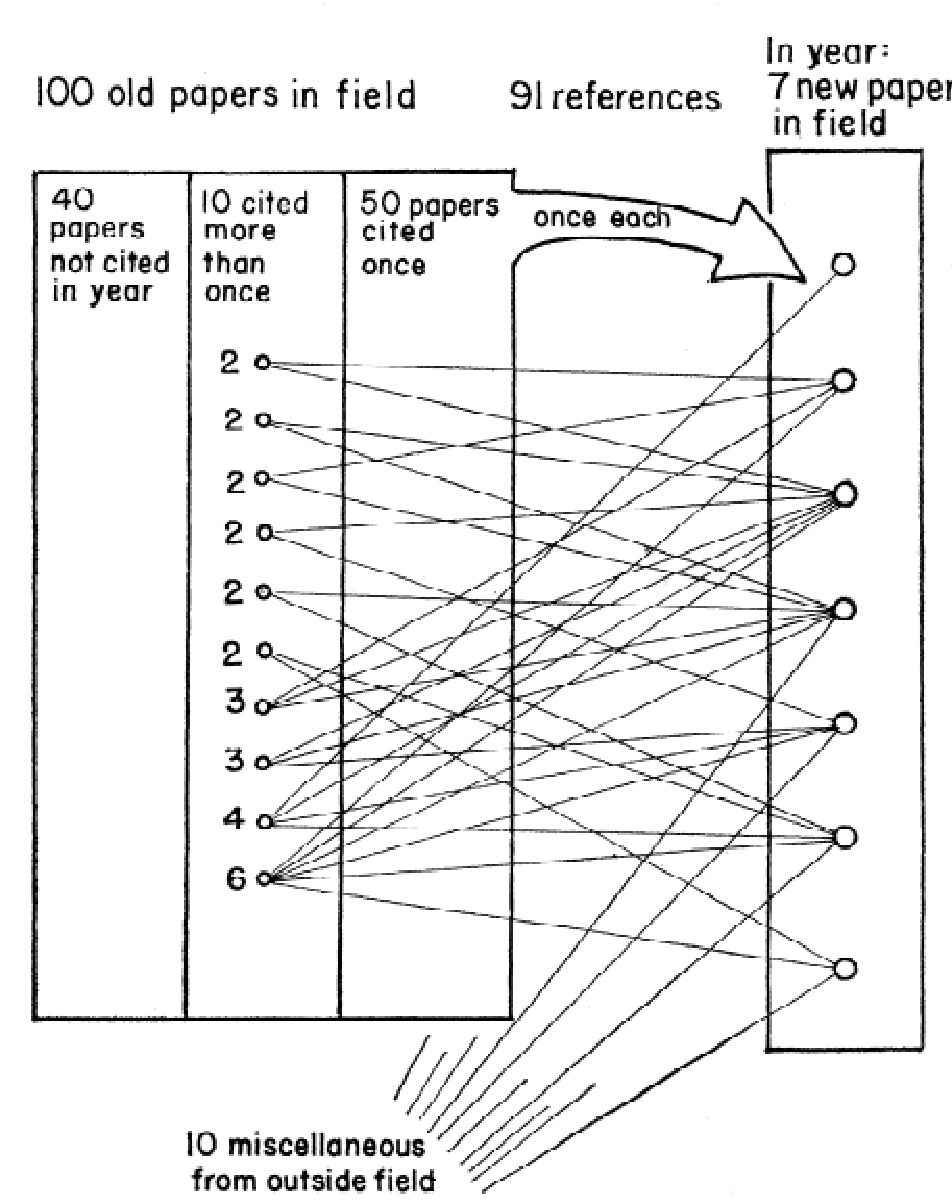
\includegraphics[height=\ht2]{desolla.pdf}%
                }%
        \else
                \setbox2\hbox{%
                        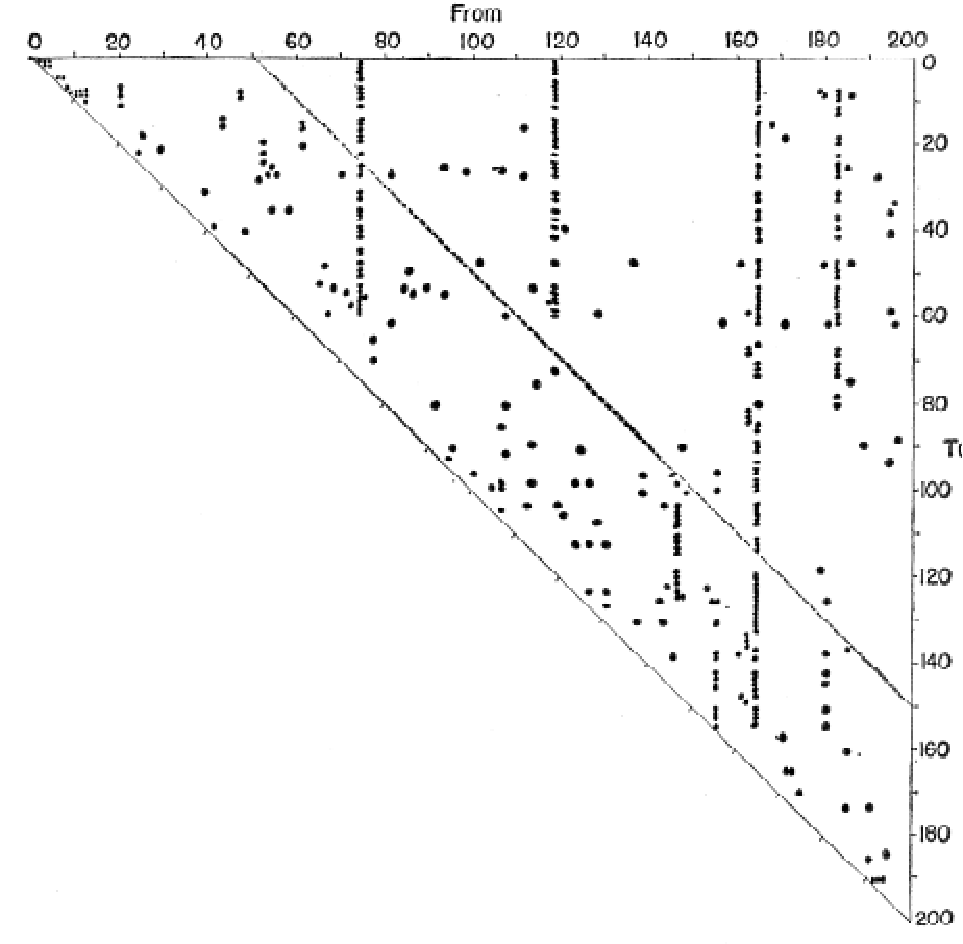
\includegraphics[height=\ht0]{desollaadjacency.pdf}%
                }%
        \fi
        \noindent
        \parbox{.45\textwidth}{%
                \centering
                \unhbox0
                \caption{Representation of citations as a network structure. Figure adapted from \cite{deSollaPrice510} with permission of The American Association for the Advancement of Science.}
                \label{fig:desolla_network}
        }%
        \hfil
        \parbox{.45\textwidth}{%
                \centering
                \unhbox2
                \caption{Representation of citations as an adjacency matrix. Figure adapted from \cite{deSollaPrice510} with permission of The American Association for the Advancement of Science.}
                \label{fig:desolla_matrix}
        }%
        
\end{figure}


What is most striking however, is that already in its origins, the study of the scientific production has required 
an analysis of science \textit{as a whole} and \textit{in time}. These key features are intrinsic properties of the entire
scientific production, since it is in the nature of science to build one's work on the top of previous ones, therefore adding a temporal dimension to
its development, as new discoveries and breakthroughs appear and link themselves to older ones. 
Since that seminal paper, the whole world, as well as the scientific one, has seen an amazing rise in technological possibilities,
which have affected heavily
the opportunities for collaborations, allowing people, as well as ideas, to move freely across the globe. 

These conditions, along with an improvement in
the economies in the post War era, has allowed science to grow at an amazing rate \cite{Larsen2010}. 
The amount of information generated by science has been growing exponentially at a rate close to a 4\% growth \textit{each year} in the last decades 
as shown in Fig.\ref{fig:growth_science}. Scientists are constantly dealing with the necessity to retrieve the latest results from their fields, which are also growing at
a fast rate; in such framework the ability to focus on the most relevant works becomes a key aspect. 
However, need for constant update requires to shift one's attention 
towards more recent scientific results, gradually discarding older ones. 

The same applies in the other direction, with scientists trying to get their latest publication known as much as possible, in order to gather \emph{attention} on their latest results. Therefore, scientists are actors in a market where the ability of reaching popularity in terms of scientific productivity has become a dominating aspect, implying that scientists/groups/institutions are all competing for attention in a market where the allocation thereof is structurally limited by one's ability to store information regarding all scientific results published in the past.


\begin{figure}[h!]
\centering
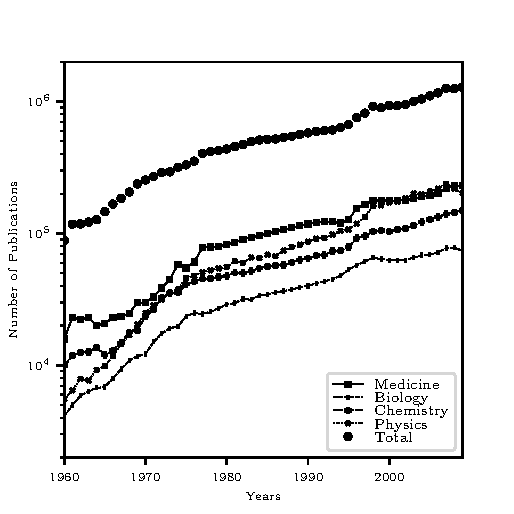
\includegraphics[width=.9\textwidth]{number_of_publications_thesis.pdf}%
\caption{Growth of publication in science and for a selected number of fields based on our ISI dataset of over 50 million publications and 600 million citations. The rate of growth can be well approximated by an exponential curve. Figure adapted from
Publication II.}\label{fig:growth_science}
\end{figure}

\section{Scope of the Thesis}
This thesis focus mainly on this temporal and cumulative aspect, investigating the changes that science has undergone in time due to its constantly changing nature.
Chapter \ref{Scientific Citations and Their Patterns} talks about the study of citation patterns, with their properties, biases and attempts at modeling them. Chapter \ref{Network Structure of Science} introduces the basic
concepts of network theory and how these concepts have been used to analyze the social and collaborative structure of science.
Chapter \ref{Science and Metrics} talks about the efforts in trying to determine the quality of scientific publications by the development of \textit{metrics}.
Finally, Chapter \ref{Results and Discussion} summarizes the content of Publications I-IV and discusses briefly how they contribute to the field of Science 
of Science.